\documentclass[]{scrartcl}
\usepackage{graphicx}

\usepackage{amsmath}
\usepackage{amsfonts}
\usepackage{amssymb}
\usepackage{float}
\usepackage{hyperref}



\hypersetup{
	colorlinks=true,
	linkcolor=blue,
	filecolor=blue,      
	urlcolor=blue,
	citecolor=blue
}


%opening
\title{Source Model Report}
\author{Trey Guest}

\begin{document}

\maketitle

\begin{abstract}

\end{abstract}
\pagebreak


\section{Coherent Source Model}

 
We define the upper limit of the FWHM of the intensity profile of the beam, $I_{FWHM}$, and the FWHM divergence of the beam, $d\theta_{FWHM}$:

\begin{table}[H]
	\caption{Modelled beam properties for 9.2 keV source generated by 100 pC beam charge.}
	\begin{center}
		\begin{tabular}{|c|c|}
			\hline 
			Electron Beam Charge (pC) & 100 \\ 
			\hline 
			Radiation Energy (keV) & 9.2 \\ 
			\hline 
			Pulse Energy (mJ) & 0.2 \\ 
			\hline 
			Pulse Duration (fs) & 102 \\ 
			\hline 
			Pulse Width ($\mu$m & 40.14 \\ 
			\hline 
			Pulse Divergence ($\mu$rad) & 5.27 \\ 
			\hline 
			
			
		\end{tabular}
	\end{center}
	
\end{table}
where
\begin{equation}\label{Eqn: FWHM upper limit}
	I_{FWHM}^{upper} = 6ln\left(\frac{7.4\times10^{3}}{E[keV]}\right),
\end{equation}
 \indent and
\begin{equation}\label{Eqn: Divergence upper limit}
	d\theta_{FWHM}^{upper} = \frac{17.2-6.4\sqrt{q[nC]}}{E^{0.85}[keV]}
\end{equation}

\noindent Plots of the profile of the beam in the real and reciprocal space are given in Figures \ref{Coherent Beam Intensity Profile R-space} and \ref{Coherent Beam Profile K-space} respectively.


\begin{figure}[H]
	\centering
	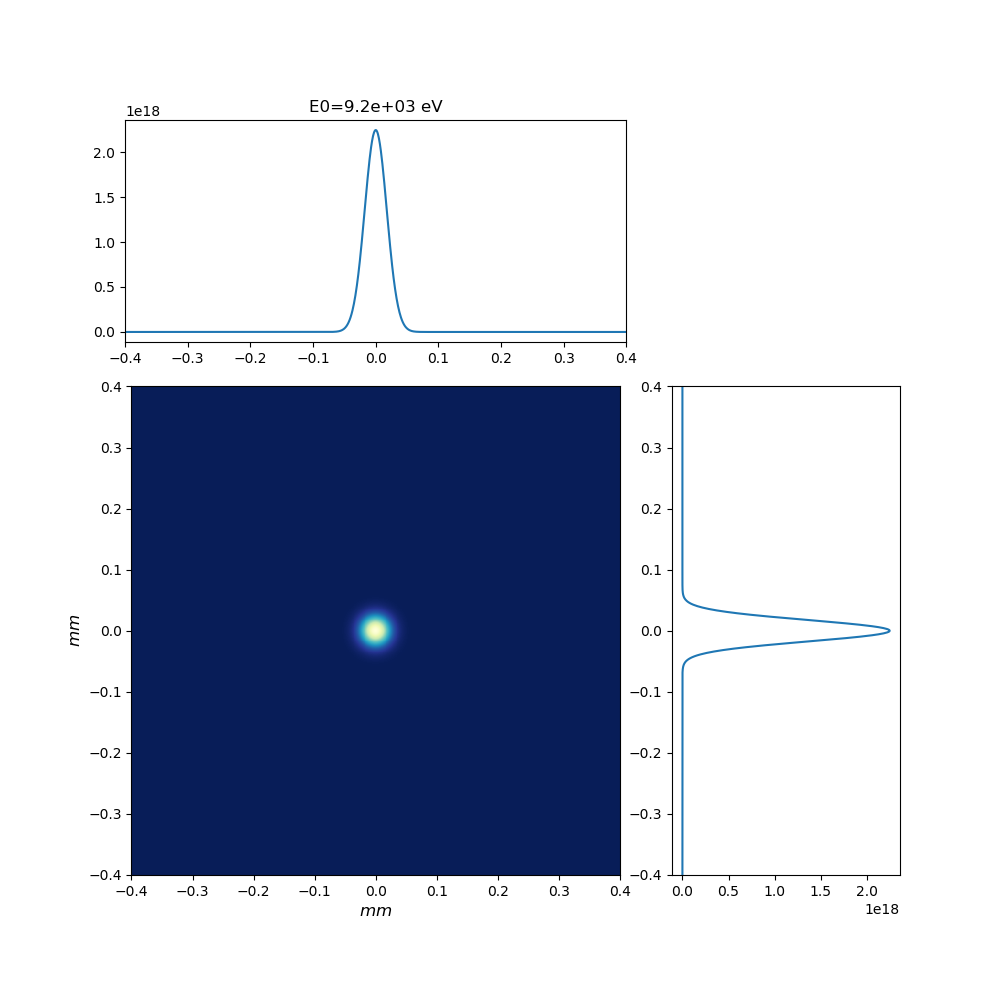
\includegraphics[width=0.5\linewidth]{srcModel_8-04-20/9200eV_100pC_intensity}
	\caption{R-space beam intensity profile of 9.2 keV source radiation at z = 0, generated from a 0.1 nC beam current.}
	\label{Coherent Beam Intensity Profile R-space}
\end{figure}

\begin{figure}[H] 
	\centering
	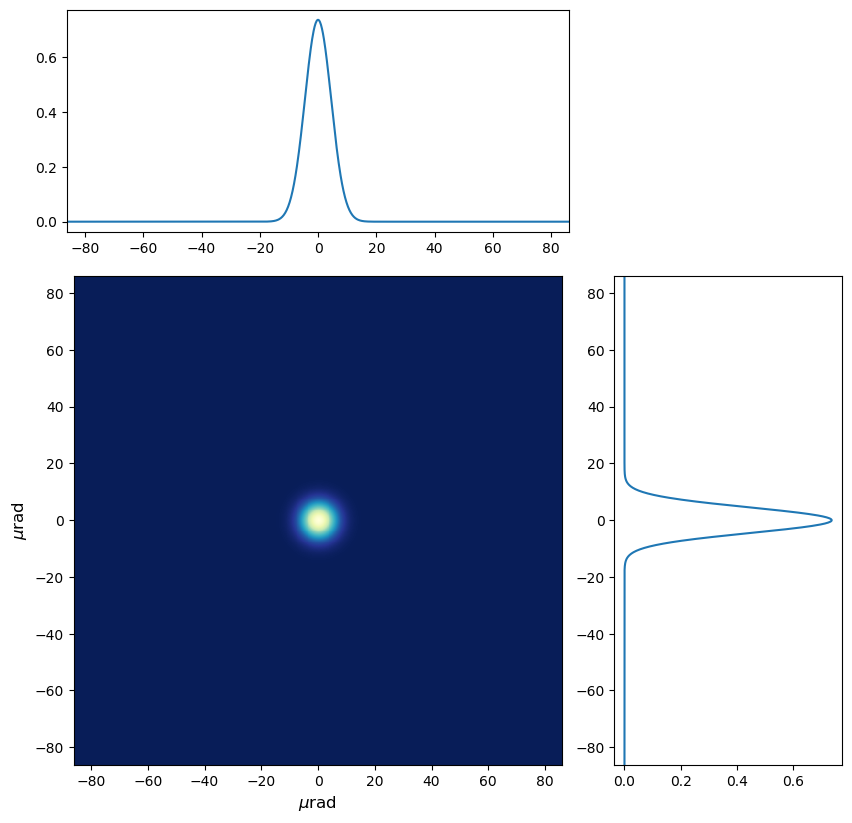
\includegraphics[width=0.5\linewidth]{srcModel_8-04-20/9200eV_100pC_kspace}
	\caption{K-space beam profile of 9.2 keV source radiation at z = 0, generated from a 0.1 nC beam current.}
	\label{Coherent Beam Profile K-space}
\end{figure}

 Following Equation \ref{Eqn: FWHM upper limit}, the energy dependent beam width is presented in Figure \ref{Fig: Energy Dependent Source Size} and demonstrates good convergence to the analytical model with increasing pixel density.\\
 
 \begin{figure}[H]
 	\centering
 	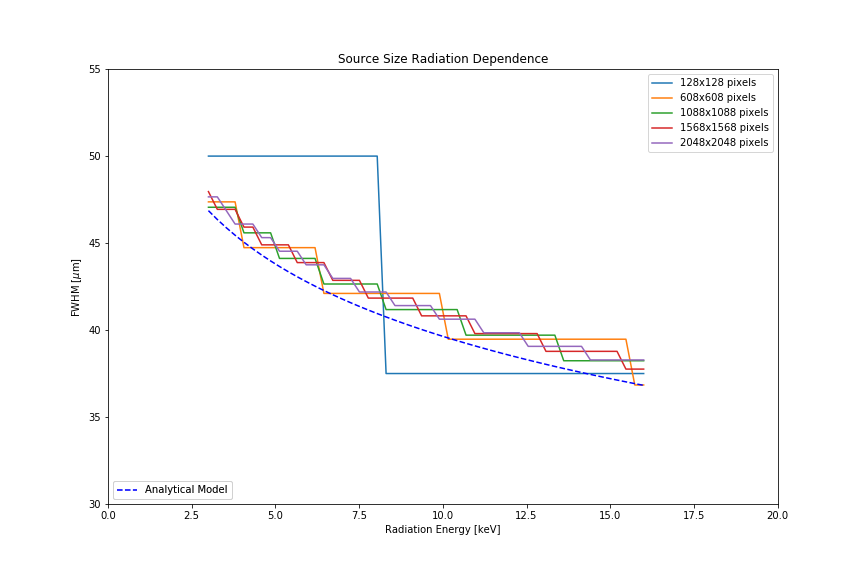
\includegraphics[width=0.7\linewidth]{srcModel_8-04-20/SourceSize_EnergyDep}
 	\caption{Comparison of simulated horizontal source width with analytical model (dashed) given in \ref{Eqn: FWHM upper limit} for increasing pixel densities.}
 	\label{Fig: Energy Dependent Source Size}
 \end{figure}

Figure \ref{Fig: FWHM Error} demonstrates only minor improvement in the convergence to the analytical result for pixel densities beyond 1024x1024. To reduce the computational load moving forward, the wavefield in the undulator exit-plane will be modelled on a 1024x1024 grid.

\begin{figure}[H]
	\centering
	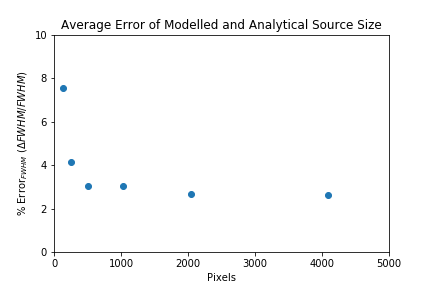
\includegraphics[width=0.7\linewidth]{srcModel_8-04-20/SourceError_pixels}
	\caption{\%Error of the measured and analytical beam profile FHWM with increasing pixel density}
		\label{Fig: FWHM Error}
	\end{figure}


Finally, a comparison of the measured and analytical source divergences is presented in Figure \ref*{Fig: Coherent Source Divergence}, showing good agreement under varying beam conditions for a wavefront size of 1024x1024 pixels.

\begin{figure}[H]
	\centering
	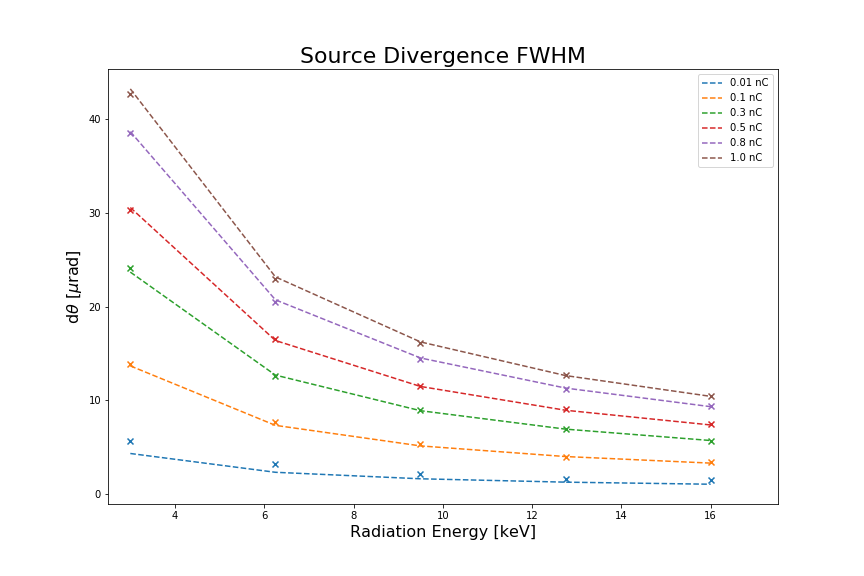
\includegraphics[width=0.7\linewidth]{srcModel_8-04-20/SourceDivergence_Energy}
	\caption{Measured (crosses) and Analytical source divergence for beam currents between 100 pC and 1 nC}
	\label{Fig: Coherent Source Divergence}
\end{figure}



\end{document}

